
%\documentclass[11pts,a4paper,amsmath,amssymb,floatfix]{article}%{report}%{book}
\documentclass[12pts,a4paper,amsmath,amssymb,floatfix]{article}%{report}%{book}
\usepackage{graphicx,wrapfig,pdfpages}% Include figure files
%\usepackage{dcolumn,enumerate}% Align table columns on decimal point
\usepackage{enumerate,enumitem}% Align table columns on decimal point
\usepackage{bm,dpfloat}% bold math
\usepackage[pdftex,bookmarks,colorlinks=true,urlcolor=rltblue,citecolor=blue]{hyperref}
\usepackage{amsfonts,amsmath,amssymb,stmaryrd,indentfirst}
\usepackage{times,psfrag}
\usepackage{natbib}
\usepackage{color}
\usepackage{units}
\usepackage{rotating}
\usepackage{multirow}


\usepackage{pifont}
\usepackage{subfigure}
\usepackage{subeqnarray}
\usepackage{ifthen}

\usepackage{supertabular}
\usepackage{moreverb}
\usepackage{listings}
\usepackage{palatino}
%\usepackage{doi}
\usepackage{longtable}
\usepackage{float}
\usepackage{perpage}
\MakeSorted{figure}
%\usepackage{pdflscape}


%\usepackage{booktabs}
%\newcommand{\ra}[1]{\renewcommand{\arraystretch}{#1}}


\definecolor{rltblue}{rgb}{0,0,0.75}


%\usepackage{natbib}
\usepackage{fancyhdr} %%%%
\pagestyle{fancy}%%%%
% with this we ensure that the chapter and section
% headings are in lowercase
%%%%\renewcommand{\chaptermark}[1]{\markboth{#1}{}}
\renewcommand{\sectionmark}[1]{\markright{\thesection\ #1}}
\fancyhf{} %delete the current section for header and footer
\fancyhead[LE,RO]{\bfseries\thepage}
\fancyhead[LO]{\bfseries\rightmark}
\fancyhead[RE]{\bfseries\leftmark}
\renewcommand{\headrulewidth}{0.5pt}
% make space for the rule
\fancypagestyle{plain}{%
\fancyhead{} %get rid of the headers on plain pages
\renewcommand{\headrulewidth}{0pt} % and the line
}

\def\newblock{\hskip .11em plus .33em minus .07em}
\usepackage{color}

%\usepackage{makeidx}
%\makeindex

\setlength\textwidth      {16.cm}
\setlength\textheight     {22.6cm}
\setlength\oddsidemargin  {-0.3cm}
\setlength\evensidemargin {0.3cm}

\setlength\headheight{14.49998pt} 
\setlength\topmargin{0.0cm}
\setlength\headsep{1.cm}
\setlength\footskip{1.cm}
\setlength\parskip{0pt}
\setlength\parindent{0pt}


%%%
%%% Headers and Footers
\lhead[] {\text{\small{EX3029 -- Chemical Thermodynamics}}} 
\rhead[] {{\text{\small{Tutorial 04 (2014/15)}}}}
%\chead[] {\text{\small{Session 2012/13}}} 
\lfoot[]{Dr Jeff Gomes}
%\cfoot[\thepage]{\thepage}
\rfoot[\text{\small{\thepage}}]{\thepage}
\renewcommand{\headrulewidth}{0.8pt}


%%%
%%% space between lines
%%%
\renewcommand{\baselinestretch}{1.5}

\newenvironment{VarDescription}[1]%
  {\begin{list}{}{\renewcommand{\makelabel}[1]{\textbf{##1:}\hfil}%
    \settowidth{\labelwidth}{\textbf{#1:}}%
    \setlength{\leftmargin}{\labelwidth}\addtolength{\leftmargin}{\labelsep}}}%
  {\end{list}}

%%%%%%%%%%%%%%%%%%%%%%%%%%%%%%%%%%%%%%%%%%%
%%%%%%                              %%%%%%%
%%%%%%      NOTATION SECTION        %%%%%%%
%%%%%%                              %%%%%%%
%%%%%%%%%%%%%%%%%%%%%%%%%%%%%%%%%%%%%%%%%%%

% Text abbreviations.
\newcommand{\ie}{{\em{i.e., }}}
\newcommand{\eg}{{\em{e.g., }}}
\newcommand{\cf}{{\em{cf., }}}
\newcommand{\wrt}{with respect to}
\newcommand{\lhs}{left hand side}
\newcommand{\rhs}{right hand side}
% Commands definining mathematical notation.

% This is for quantities which are physically vectors.
\renewcommand{\vec}[1]{{\mbox{\boldmath$#1$}}}
% Physical rank 2 tensors
\newcommand{\tensor}[1]{\overline{\overline{#1}}}
% This is for vectors formed of the value of a quantity at each node.
\newcommand{\dvec}[1]{\underline{#1}}
% This is for matrices in the discrete system.
\newcommand{\mat}[1]{\mathrm{#1}}


\DeclareMathOperator{\sgn}{sgn}
\newtheorem{thm}{Theorem}[section]
\newtheorem{lemma}[thm]{Lemma}

%\newcommand\qed{\hfill\mbox{$\Box$}}
\newcommand{\re}{{\mathrm{I}\hspace{-0.2em}\mathrm{R}}}
\newcommand{\inner}[2]{\langle#1,#2\rangle}
\renewcommand\leq{\leqslant}
\renewcommand\geq{\geqslant}
\renewcommand\le{\leqslant}
\renewcommand\ge{\geqslant}
\renewcommand\epsilon{\varepsilon}
\newcommand\eps{\varepsilon}
\renewcommand\phi{\varphi}
\newcommand{\bmF}{\vec{F}}
\newcommand{\bmphi}{\vec{\phi}}
\newcommand{\bmn}{\vec{n}}
\newcommand{\bmns}{{\textrm{\scriptsize{\boldmath $n$}}}}
\newcommand{\bmi}{\vec{i}}
\newcommand{\bmj}{\vec{j}}
\newcommand{\bmk}{\vec{k}}
\newcommand{\bmx}{\vec{x}}
\newcommand{\bmu}{\vec{u}}
\newcommand{\bmv}{\vec{v}}
\newcommand{\bmr}{\vec{r}}
\newcommand{\bma}{\vec{a}}
\newcommand{\bmg}{\vec{g}}
\newcommand{\bmU}{\vec{U}}
\newcommand{\bmI}{\vec{I}}
\newcommand{\bmq}{\vec{q}}
\newcommand{\bmT}{\vec{T}}
\newcommand{\bmM}{\vec{M}}
\newcommand{\bmtau}{\vec{\tau}}
\newcommand{\bmOmega}{\vec{\Omega}}
\newcommand{\pp}{\partial}
\newcommand{\kaptens}{\tensor{\kappa}}
\newcommand{\tautens}{\tensor{\tau}}
\newcommand{\sigtens}{\tensor{\sigma}}
\newcommand{\etens}{\tensor{\dot\epsilon}}
\newcommand{\ktens}{\tensor{k}}
\newcommand{\half}{{\textstyle \frac{1}{2}}}
\newcommand{\tote}{E}
\newcommand{\inte}{e}
\newcommand{\strt}{\dot\epsilon}
\newcommand{\modu}{|\bmu|}
% Derivatives
\renewcommand{\d}{\mathrm{d}}
\newcommand{\D}{\mathrm{D}}
\newcommand{\ddx}[2][x]{\frac{\d#2}{\d#1}}
\newcommand{\ddxx}[2][x]{\frac{\d^2#2}{\d#1^2}}
\newcommand{\ddt}[2][t]{\frac{\d#2}{\d#1}}
\newcommand{\ddtt}[2][t]{\frac{\d^2#2}{\d#1^2}}
\newcommand{\ppx}[2][x]{\frac{\partial#2}{\partial#1}}
\newcommand{\ppxx}[2][x]{\frac{\partial^2#2}{\partial#1^2}}
\newcommand{\ppt}[2][t]{\frac{\partial#2}{\partial#1}}
\newcommand{\pptt}[2][t]{\frac{\partial^2#2}{\partial#1^2}}
\newcommand{\DDx}[2][x]{\frac{\D#2}{\D#1}}
\newcommand{\DDxx}[2][x]{\frac{\D^2#2}{\D#1^2}}
\newcommand{\DDt}[2][t]{\frac{\D#2}{\D#1}}
\newcommand{\DDtt}[2][t]{\frac{\D^2#2}{\D#1^2}}
% Norms
\newcommand{\Ltwo}{\ensuremath{L_2} }
% Basis functions
\newcommand{\Qone}{\ensuremath{Q_1} }
\newcommand{\Qtwo}{\ensuremath{Q_2} }
\newcommand{\Qthree}{\ensuremath{Q_3} }
\newcommand{\QN}{\ensuremath{Q_N} }
\newcommand{\Pzero}{\ensuremath{P_0} }
\newcommand{\Pone}{\ensuremath{P_1} }
\newcommand{\Ptwo}{\ensuremath{P_2} }
\newcommand{\Pthree}{\ensuremath{P_3} }
\newcommand{\PN}{\ensuremath{P_N} }
\newcommand{\Poo}{\ensuremath{P_1P_1} }
\newcommand{\PoDGPt}{\ensuremath{P_{-1}P_2} }

\newcommand{\metric}{\tensor{M}}
\newcommand{\configureflag}[1]{\texttt{#1}}

% Units
\newcommand{\m}[1][]{\unit[#1]{m}}
\newcommand{\km}[1][]{\unit[#1]{km}}
\newcommand{\s}[1][]{\unit[#1]{s}}
\newcommand{\invs}[1][]{\unit[#1]{s}\ensuremath{^{-1}}}
\newcommand{\ms}[1][]{\unit[#1]{m\ensuremath{\,}s\ensuremath{^{-1}}}}
\newcommand{\mss}[1][]{\unit[#1]{m\ensuremath{\,}s\ensuremath{^{-2}}}}
\newcommand{\K}[1][]{\unit[#1]{K}}
\newcommand{\PSU}[1][]{\unit[#1]{PSU}}
\newcommand{\Pa}[1][]{\unit[#1]{Pa}}
\newcommand{\kg}[1][]{\unit[#1]{kg}}
\newcommand{\rads}[1][]{\unit[#1]{rad\ensuremath{\,}s\ensuremath{^{-1}}}}
\newcommand{\kgmm}[1][]{\unit[#1]{kg\ensuremath{\,}m\ensuremath{^{-2}}}}
\newcommand{\kgmmm}[1][]{\unit[#1]{kg\ensuremath{\,}m\ensuremath{^{-3}}}}
\newcommand{\Nmm}[1][]{\unit[#1]{N\ensuremath{\,}m\ensuremath{^{-2}}}}

% Dimensionless numbers
\newcommand{\dimensionless}[1]{\mathrm{#1}}
\renewcommand{\Re}{\dimensionless{Re}}
\newcommand{\Ro}{\dimensionless{Ro}}
\newcommand{\Fr}{\dimensionless{Fr}}
\newcommand{\Bu}{\dimensionless{Bu}}
\newcommand{\Ri}{\dimensionless{Ri}}
\renewcommand{\Pr}{\dimensionless{Pr}}
\newcommand{\Pe}{\dimensionless{Pe}}
\newcommand{\Ek}{\dimensionless{Ek}}
\newcommand{\Gr}{\dimensionless{Gr}}
\newcommand{\Ra}{\dimensionless{Ra}}
\newcommand{\Sh}{\dimensionless{Sh}}
\newcommand{\Sc}{\dimensionless{Sc}}


% Journals
\newcommand{\IJHMT}{{\it International Journal of Heat and Mass Transfer}}
\newcommand{\NED}{{\it Nuclear Engineering and Design}}
\newcommand{\ICHMT}{{\it International Communications in Heat and Mass Transfer}}
\newcommand{\NET}{{\it Nuclear Engineering and Technology}}
\newcommand{\HT}{{\it Heat Transfer}}   
\newcommand{\IJHT}{{\it International Journal for Heat Transfer}}

\newcommand{\frc}{\displaystyle\frac}

\newlist{ExList}{enumerate}{1}
\setlist[ExList,1]{label={\bf Example 1.} {\bf \arabic*}}

\newlist{ProbList}{enumerate}{1}
\setlist[ProbList,1]{label={\bf Problem 1.} {\bf \arabic*}}

%%%%%%%%%%%%%%%%%%%%%%%%%%%%%%%%%%%%%%%%%%%
%%%%%%                              %%%%%%%
%%%%%% END OF THE NOTATION SECTION  %%%%%%%
%%%%%%                              %%%%%%%
%%%%%%%%%%%%%%%%%%%%%%%%%%%%%%%%%%%%%%%%%%%


% Cause numbering of subsubsections. 
%\setcounter{secnumdepth}{8}
%\setcounter{tocdepth}{8}

\setcounter{secnumdepth}{4}%
\setcounter{tocdepth}{4}%


\begin{document}



\begin{enumerate}[label=\bfseries Problem \arabic*:]

%%%
%%% Johannes T4Q1
%%%
\item\label{Tut04:Steam1} Steam entering a turbine at 4MPa and 400$^{\circ}$C expands reversibly and adiabatically.
\begin{enumerate}
\item For what discharge pressure is the exit stream a saturated vapour?
\item Determine the steam quality for a discharge pressure of 250 kPa.
\item Sketch both processes in a $TS$ diagram.
\end{enumerate}

%%%
%%% Johannes Solved Problem
%%%
\item\label{Tut04:Steam2} Superheated steam originally at P$_{1}$= 1000kPa and T$_{1}$ = 250$^{\circ}$C expands through a nozzle to an exhaust pressure P$_{2}$ =  200 kPa. What is the downstream state of the steam and the change in enthalpy assuming a reversible and adiabatic process?

%%%
%%% SM&VN 6.22
%%%
\item\label{solutions} A liquid-vapour water system is in equilibrium at 80 bar. The system consists of equal volumes of liquid and vapour with total volume $\left(V^{T}\right)$ of 0.15 m$^{3}$. Calculate the total enthalpy $\left(H^{T}\right)$ and $\left(S^{T}\right)$. 

%%%
%%%
%%%
\item\label{prove} For $\beta = \frc{1}{V}\left(\frc{\partial V}{\partial T}\right)_{P}$ (volume expansivity) and $\kappa = -\frc{1}{V}\left(\frc{\partial V}{\partial P}\right)_{T}$ (isothermal compressibility), demonstrate that $\left(\frc{\partial\beta}{\partial P}\right)_{T} = -\left(\frc{\partial\kappa}{\partial T}\right)_{P}$. Hint: consider $V=V\left(T,P\right)$.

%%%
%%% Jeff Solved Exampple 1
%%%
\item\label{SolvedExample2} Steam is produced in a boiler at 60 bar and 335$^{\circ}$C . The fluid is driven into a turbine where an isentropic expansion take place with efficiency of 75$\%$. Before re-vaporisation in the boiler, the fluid is condensed in a heat exchanger, where the extracted energy is used to heat up a stream of NH$_{3}$ at 15$^{\circ}$C. The mass flow rate of water and NH$_{3}$ are 20 and 220 kg.s$^{-1}$, respectively. Assume that the pump has 100$\%$ of efficiency.
\begin{center}
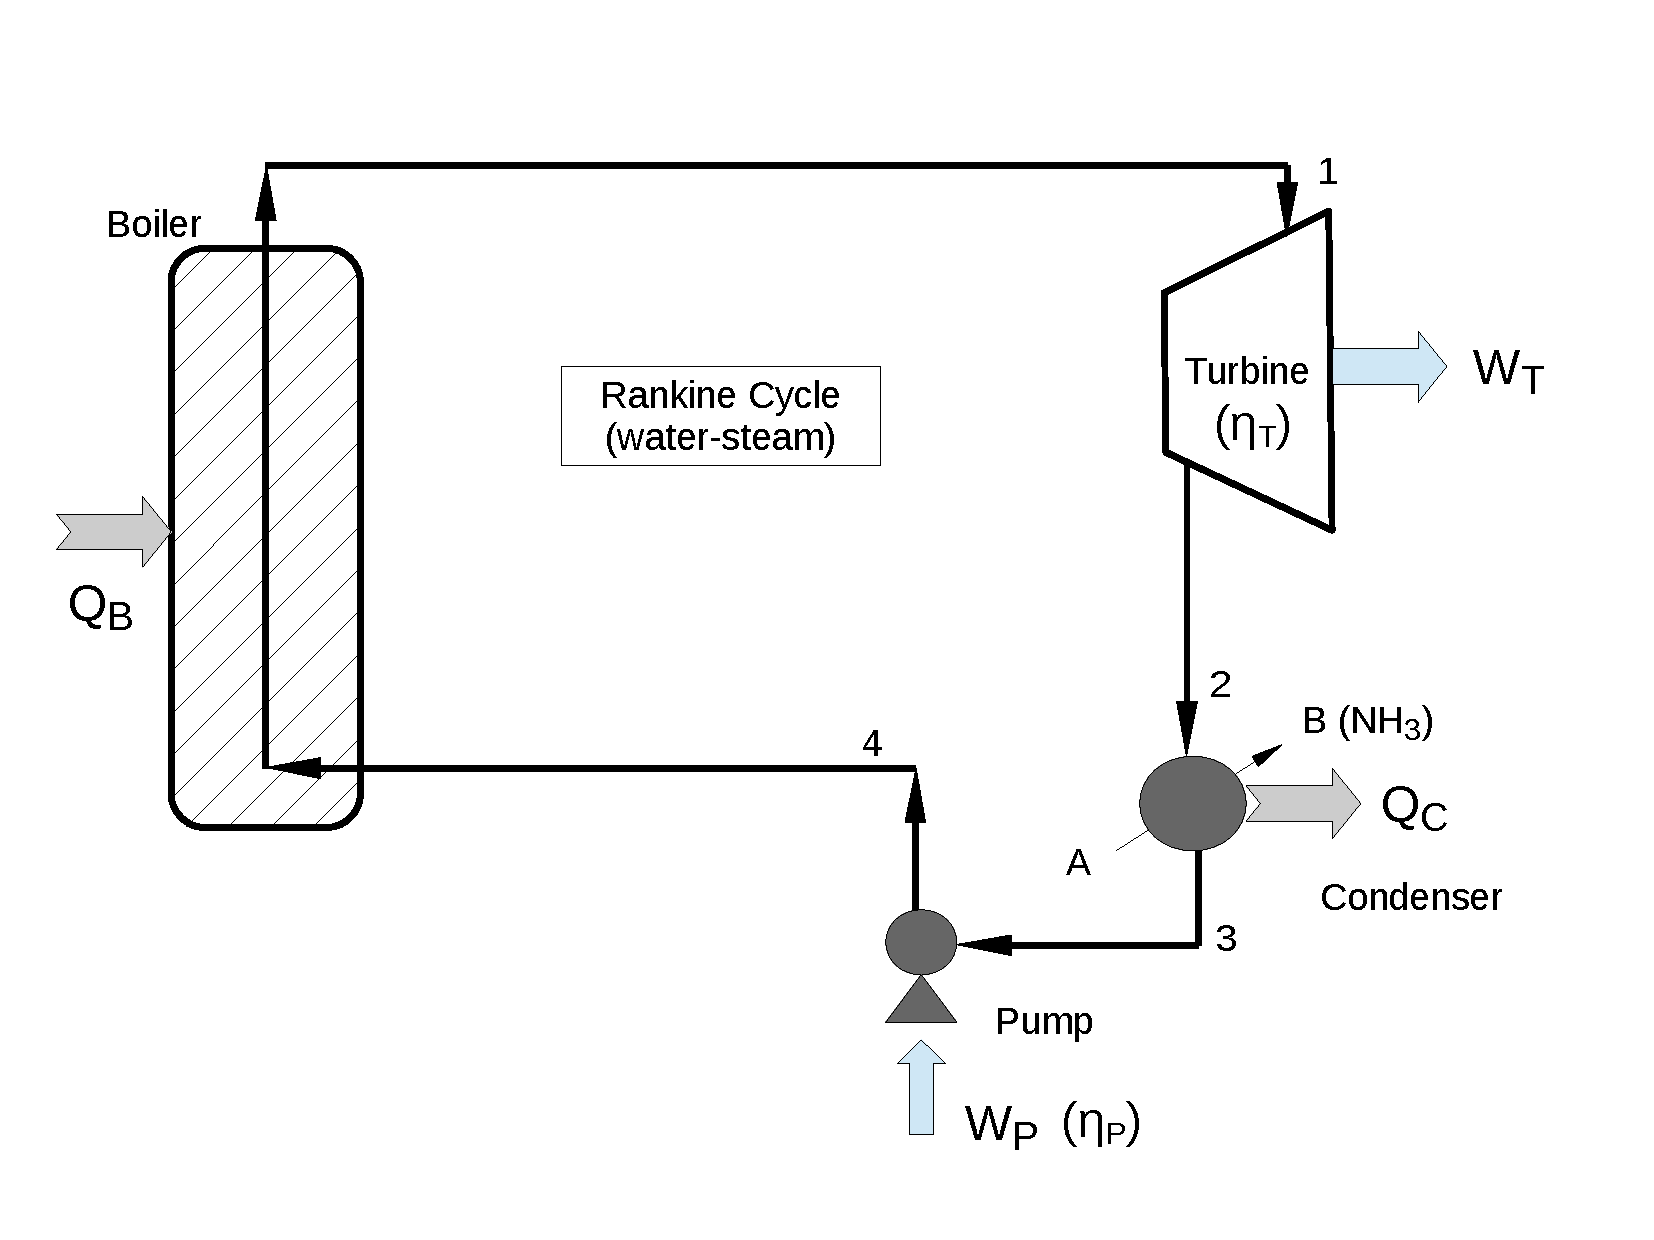
\includegraphics[width=12.cm,height=8.cm,clip]{./Pics/RankineCycle2}
%\caption{ Reheat and regenerative Rankine cycle with 2 turbines.}
\label{exam_mod02_rankinecycle}
\end{center}
\begin{enumerate}
\item Calculate (a-n) in the table below.
\item Calculate the power produced in the turbine $\left(\dot{W}_{T}\right)$ and required in the pump $\left(\dot{W}_{P}\right)$.
\item Calculate the heat given to the system in the boiler $\left(\dot{Q}_{B}\right)$ and extracted in the condenser $\left(\dot{Q}_{C}\right)$.
\item Calculate the efficiency of the cycle $\left(\eta_{\text{cycle}}=\frc{\dot{W}_{\text{net}}}{\dot{Q}_{B}}\right)$
\end{enumerate}
\begin{center}
\begin{tabular} {||c | c c c c c c || }
\hline\hline
{\bf Stage} & {\bf P}    & {\bf T}        & {\bf State}    & {\bf H}             & {\bf S}                 &  {\bf Quality of the} \\
            & {\bf (bar)}& {\bf ($^{o}$C)} &               & {\bf (kJ.kg$^{-1}$)} & {\bf (kJ.(kg.K)$^{-1}$)} &  {\bf vapour $\left(x_{i}\right)$} \\
\hline\hline
 {\bf 1 }   & 60         & 335            &   {\bf (a)}    & {\bf (b)}           & {\bf (c)}               &   --          \\
 {\bf 2 }   & 4.50       &  --            &   wet vapour   & {\bf (d)}           & {\bf (e)}               &   {\bf (f)}    \\
 {\bf 3 }   & {\bf(g)}   &                &   sat. liquid  & {\bf (h)}           & {\bf (i)}               &   --            \\
 {\bf 4 }   & {\bf(j)}   &                &   {\bf (k)}    & {\bf (l)}           & {\bf (m)}               &   --            \\
 {\bf A }   & --         & 15             &   --           & --                  & --                      &   --     \\
 {\bf B }   & --         & {\bf (n)}      &   --           & --                  & --                      &   --         \\
 \hline\hline
\end{tabular}
\end{center}




%%%
%%% Jeff Solved Example 2
%%% 
\item\label{SolvedExample2} Evaluate $\left(\frc{\partial S}{\partial V}\right)_{T}$ for  water-vapour at 240$^{\circ}$C and specific volume of 0.4646 m$^{3}$.kg$^{-1}$. Use,
\begin{enumerate}
\item Peng-Robinson EOS;
\item Redlich-Kwong EOS.
\end{enumerate}
Given: T$_{c}$ 647.096 K, P$_{c}$ = 220.6 bar and $\omega$ = 0.344.

\clearpage


\end{enumerate} 
%{
%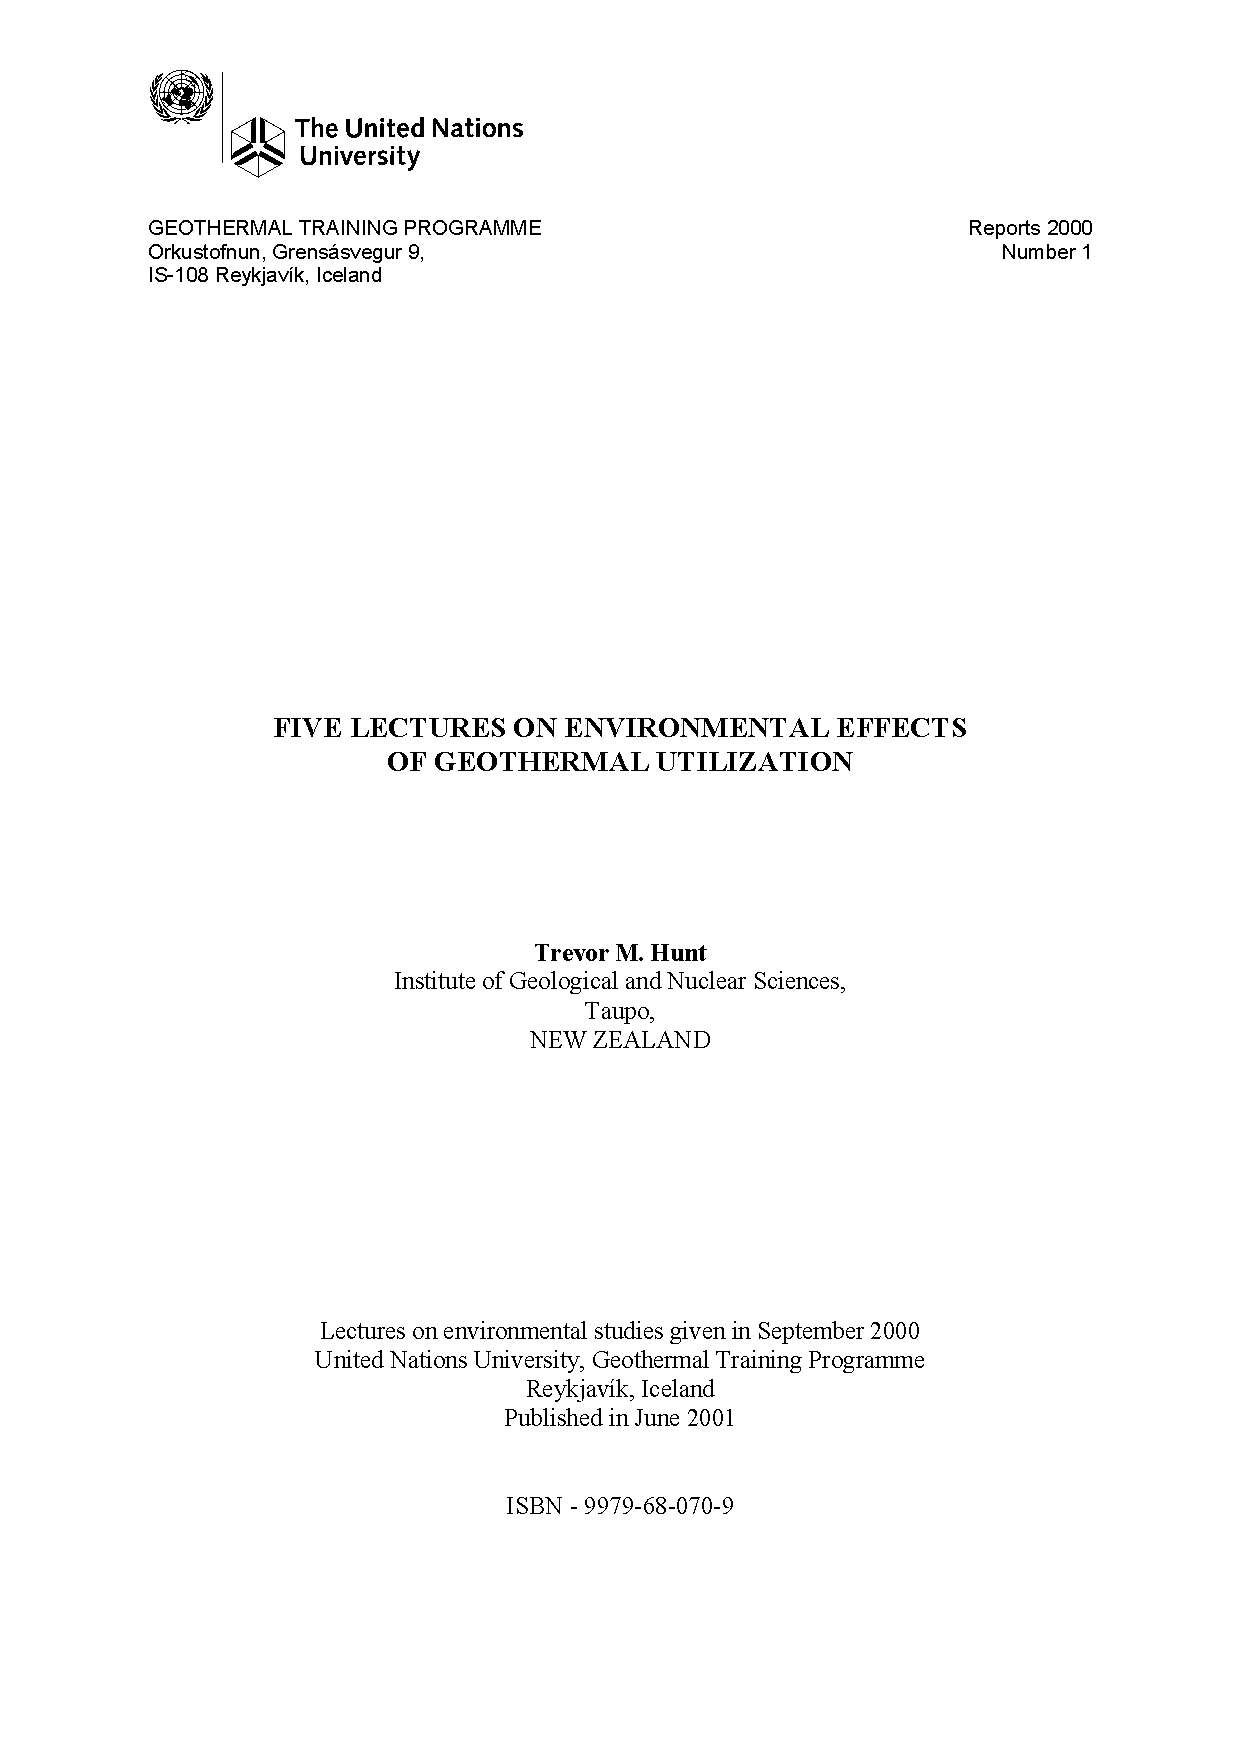
\includepdf[pages=-,fitpaper, angle=0]{./HuntSelect.pdf}
%}

\end{document}
